\documentclass[12pt]{article}
%%---------------------------------------------------------------------
% packages
% geometry
\usepackage{geometry}
% font
\usepackage{fontspec}
\defaultfontfeatures{Mapping=tex-text}  %%如果没有它,会有一些 tex 特殊字符无法正常使用,比如连字符。
\usepackage{xunicode,xltxtra}
\usepackage[BoldFont,SlantFont,CJKnumber,CJKchecksingle]{xeCJK}  % \CJKnumber{12345}: 一万二千三百四十五
\usepackage{CJKfntef}  %%实现对汉字加点、下划线等。
\usepackage{pifont}  % \ding{}
% math
\usepackage{amsmath,amsfonts,amssymb}
% color
\usepackage{color}
\usepackage{xcolor}
\definecolor{EYE}{RGB}{199,237,204}
\definecolor{FLY}{RGB}{128,0,128}
\definecolor{ZHY}{RGB}{139,0,255}
% graphics
\usepackage[americaninductors,europeanresistors]{circuitikz}
\usepackage{tikz}
\usetikzlibrary{positioning,arrows,shadows,shapes,calc,mindmap,trees,backgrounds}  % placements=positioning
\usepackage{graphicx}  % \includegraphics[]{}
\usepackage{subfigure}  %%图形或表格并排排列
% table
\usepackage{colortbl,dcolumn}  %% 彩色表格
\usepackage{multirow}
\usepackage{multicol}
\usepackage{booktabs}
% code
\usepackage{fancyvrb}
\usepackage{listings}
% title
\usepackage{titlesec}
% head/foot
\usepackage{fancyhdr}
% ref
\usepackage{hyperref} %生成可链接目录
% pagecolor
\usepackage[pagecolor={EYE}]{pagecolor}
% tightly-packed lists
\usepackage{mdwlist}
\usepackage{verbatim}%comment命令的注释包
\usepackage{styles/iplouccfg}
\usepackage{styles/zhfontcfg}
\usepackage{styles/iplouclistings}
%%---------------------------------------------------------------------
% settings
% geometry
\geometry{left=2cm,right=1cm,top=2cm,bottom=2cm}  %设置 上、左、下、右 页边距
\linespread{1.5} %行间距
% font
\setCJKmainfont{Adobe Kaiti Std}
%\setmainfont[BoldFont=Adobe Garamond Pro Bold]{Apple Garamond}  % 英文字体
%\setmainfont[BoldFont=Adobe Garamond Pro Bold,SmallCapsFont=Apple Garamond,SmallCapsFeatures={Scale=0.7}]{Apple Garamond}  %%苹果字体没有SmallCaps
\setCJKmonofont{Adobe Fangsong Std}
% graphics
\graphicspath{{figures/}}
\tikzset{
    % Define standard arrow tip
    >=stealth',
    % Define style for boxes
    punkt/.style={
           rectangle,
           rounded corners,
           draw=black, very thick,
           text width=6.5em,
           minimum height=2em,
           text centered},
    % Define arrow style
    pil/.style={
           ->,
           thick,
           shorten <=2pt,
           shorten >=2pt,},
    % Define style for FlyZhyBall
    FlyZhyBall/.style={
      circle,
      minimum size=6mm,
      inner sep=0.5pt,
      ball color=red!50!blue,
      text=white,},
    % Define style for FlyZhyRectangle
    FlyZhyRectangle/.style={
      rectangle,
      rounded corners,
      minimum size=6mm,
      ball color=red!50!blue,
      text=white,},
    % Define style for zhyfly
    zhyfly/.style={
      rectangle,
      rounded corners,
      minimum size=6mm,
      ball color=red!25!blue,
      text=white,},
    % Define style for new rectangle
    nrectangle/.style={
      rectangle,
      draw=#1!50,
      fill=#1!20,
      minimum size=5mm,
      inner sep=0.1pt,}
}
\ctikzset{
  bipoles/length=.8cm
}
% code
\lstnewenvironment{VHDLcode}[1][]{%
  \lstset{
    basicstyle=\footnotesize\ttfamily\color{black},%
    columns=flexible,%
    framexleftmargin=.7mm,frame=shadowbox,%
    rulesepcolor=\color{blue},%
%    frame=single,%
    backgroundcolor=\color{yellow!20},%
    xleftmargin=1.2\fboxsep,%
    xrightmargin=.7\fboxsep,%
    numbers=left,numberstyle=\tiny\color{blue},%
    numberblanklines=false,numbersep=7pt,%
    language=VHDL%
    }\lstset{#1}}{}
\lstnewenvironment{VHDLmiddle}[1][]{%
  \lstset{
    basicstyle=\scriptsize\ttfamily\color{black},%
    columns=flexible,%
    framexleftmargin=.7mm,frame=shadowbox,%
    rulesepcolor=\color{blue},%
%    frame=single,%
    backgroundcolor=\color{yellow!20},%
    xleftmargin=1.2\fboxsep,%
    xrightmargin=.7\fboxsep,%
    numbers=left,numberstyle=\tiny\color{blue},%
    numberblanklines=false,numbersep=7pt,%
    language=VHDL%
    }\lstset{#1}}{}
\lstnewenvironment{VHDLsmall}[1][]{%
  \lstset{
    basicstyle=\tiny\ttfamily\color{black},%
    columns=flexible,%
    framexleftmargin=.7mm,frame=shadowbox,%
    rulesepcolor=\color{blue},%
%    frame=single,%
    backgroundcolor=\color{yellow!20},%
    xleftmargin=1.2\fboxsep,%
    xrightmargin=.7\fboxsep,%
    numbers=left,numberstyle=\tiny\color{blue},%
    numberblanklines=false,numbersep=7pt,%
    language=VHDL%
    }\lstset{#1}}{}
% pdf
\hypersetup{pdfauthor={Haiyong Zheng},%
            pdftitle={Title},%
            CJKbookmarks=true,%
            bookmarksnumbered=true,%
            bookmarksopen=false,%
            plainpages=false,%
            colorlinks=true,%
            citecolor=green,%
            filecolor=magenta,%
            linkcolor=cyan,%red(default)
            urlcolor=cyan}
% section
%http://tex.stackexchange.com/questions/34288/how-to-place-a-shaded-box-around-a-section-label-and-name
\newcommand\titlebar{%
\tikz[baseline,trim left=3.1cm,trim right=3cm] {
    \fill [cyan!25] (2.5cm,-1ex) rectangle (\textwidth+3.1cm,2.5ex);
    \node [
        fill=cyan!60!white,
        anchor= base east,
        rounded rectangle,
        minimum height=3.5ex] at (3cm,0) {
        \textbf{\thesection.}
    };
}%
}
\titleformat{\section}{\Large\bf\color{blue}}{\titlebar}{0.1cm}{}
% head/foot
\setlength{\headheight}{15pt}
\pagestyle{fancy}
\fancyhf{}
\numberwithin{equation}{section}%%公式与章节关联
%\lhead{\color{black!50!green}2014年秋季学期}
\chead{\color{black!50!green}Machine Learning Note}
%\rhead{\color{black!50!green}通信电子电路}
\lfoot{\color{blue!50!green}常琳}
%\cfoot{\color{blue!50!green}\href{http://vision.ouc.edu.cn/~zhenghaiyong}{CVBIOUC}}
\rfoot{\color{blue!50!green}$\cdot$\ \thepage\ $\cdot$}
\renewcommand{\headrulewidth}{0.4pt}
\renewcommand{\footrulewidth}{0.4pt}

%%---------------------------------------------------------------------
\begin{document}
%%---------------------------------------------------------------------
%%---------------------------------------------------------------------
% \titlepage
\title{\vspace{-2em}Machine Learning Note\vspace{-0.7em}}
\author{}
\date{}
%%---------------------------------------------------------------------
\maketitle\thispagestyle{fancy}
%%---------------------------------------------------------------------
\maketitle
\tableofcontents 
%---------------------------------------------------------------------

\linespread{1.5} %行间距

%=======================================================================

\section{模型评估与选择}

\subsection{经验误差与过拟合}

学习器在训练集上的误差称为``训练误差"或``经验误差"(empirical error),在新样本上的误差称为``泛化误差"(generalization error).

``过拟合":训练样本学的太好,泛化性能下降      /quad 是机器学习的关键障碍,无法彻底避免

``欠拟合":是指对训练样本的一般性质尚未学好

\subsection{评估方法}

现实中要考虑时间开销,存储开销(这俩也算是降维兴起的原因),可解释性等方面因素,这里只考虑泛化误差.

\subsubsection{留出法}

直接将数据集D划分为两个互斥的集合,训练集S和测试集T.训练/测试集的划分要尽量保持数据分布的一致性.

单次使用留出法得到的估计结果不够稳定可靠,一般采用多次随机划分,重复试验取平均值作为评估结果.

\subsubsection{交叉验证法}

先将数据集D划分成k个(k折)大小相似的互斥子集,每个子集都尽可能保持数据分布的一致性,即从D中通过分层采样得到. 然后每次用k-1个子集的并集作为训练集, 余下子集作为测试集,进行k次训练和测试,最终返回的是k个测试结果的均值.

为减小因样本划分不同而引入的差别,k折要随机用不同的划分重复p次,最终评估结果是p次k折交叉验证结果的均值.

假定D包含m个样本,若令k=m, 得到特例: 留一法 (Leave-One-Out, LOO)

%%----------------------------------------------------------------------------------------------------------------------------------------------------------------------------------------------------
\section{支持向量机}

\subsection{间隔与支持向量}

样本空间中划分超平面:

\begin{equation}
\boldsymbol{\omega}^{T}\boldsymbol{x}+b=0
\end{equation}

\boldmath$\omega$  \unboldmath = $\{\omega_{1};\omega_{2};\ldots \omega_{d}\}$ 为法向量,决定超平面的方向; $b$ 为位移项,决定超平面与原点之间的距离.

样本空间任一点\boldmath$x$到超平面 \boldmath($\omega$, \unboldmath$b$) 的距离:

\begin{equation}
r=\dfrac{\mid \boldsymbol{\omega}^{T}\boldsymbol{x}+b \mid}{\parallel \boldsymbol{\omega} \parallel}
\end{equation}

设超平面 \boldmath($\omega$, \unboldmath$b$)能将训练样本正确分类,即对于超平面 \boldmath($x_{i}$, \unboldmath$y_{i}$) $\in D$,若$y_{i}=+1$, 则有
$ \boldsymbol{\omega}^{T}\boldsymbol{x}+b>0$; 若 $y_{i}=-1$, $ \boldsymbol{\omega}^{T}\boldsymbol{x}+b<0$. 另

\begin{equation}
\label{6-3}
 \left\{ \begin{array}{ll}
 \boldsymbol{\omega}^{T}\boldsymbol{x}_{i}+b \geqslant +1 & \textrm{ $y_{i}=+1$}\\
\boldsymbol{\omega}^{T}\boldsymbol{x}_{i}+b \leqslant -1  &  \textrm{ $y_{i}=-1$}\\
\end{array} \right.
\end{equation}

如图\ref{6-2}, 距离超平面最近的几个样本点使式\ref{6.3}的等号成立,每个样本点对应一个特征向量, 他们被称为``支持向量", 两个异类支持向量到超平面的距离和:

\begin{equation}
\gamma=\frac{2}{\parallel \boldsymbol{\omega} \parallel}
\end{equation}
称为``间隔"(margin).
\begin{figure}
\centering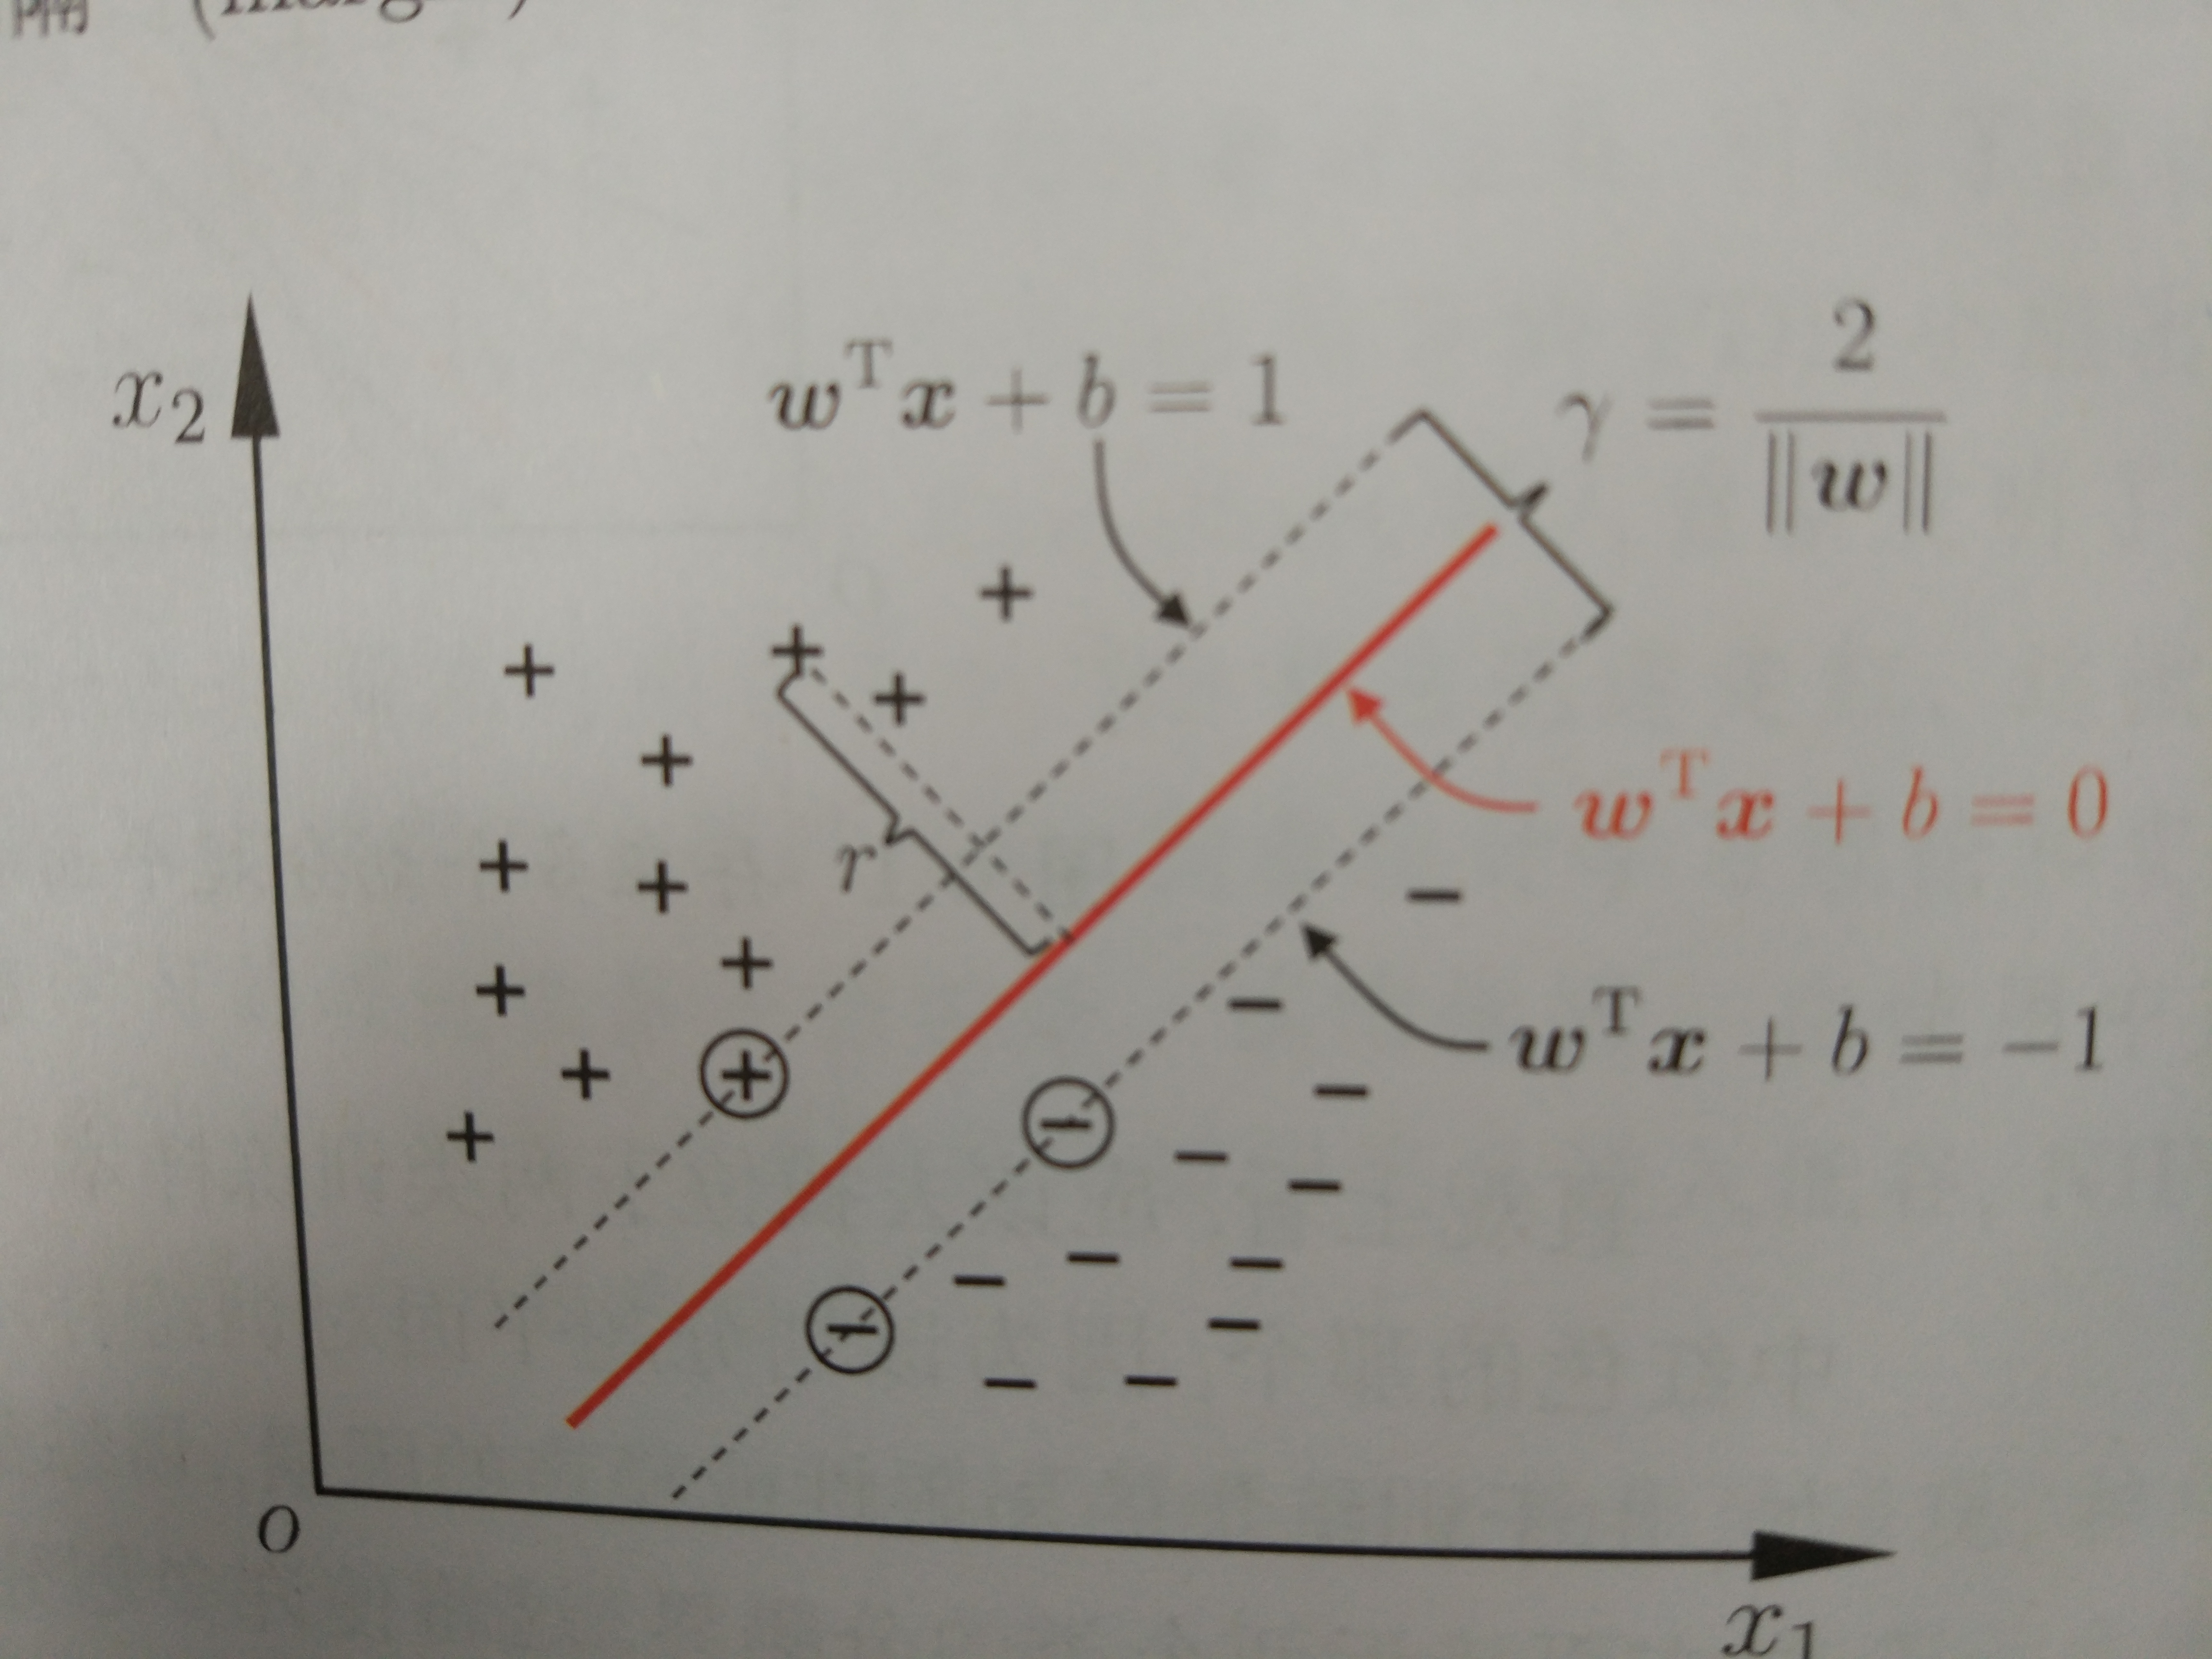
\includegraphics[width=5in]{6-2.jpg}
\caption{支持向量与间隔}
\label{6-2}
\end{figure}

欲找到具有``最大间隔"(maximum margin)的划分超平面,即



\begin{equation}
\begin{split}        %换行 
 {\underset{\boldsymbol{\omega},b}{max}} \quad \frac{2}{\parallel \boldsymbol{\omega} \parallel}  \\
 s.t. \quad y_{i}(\boldsymbol{\omega}^{T}\boldsymbol{x}_{i}+b) \geqslant 1, \quad i= 1,2, \ldots ,m.
\end{split}
\label{6-5}
\end{equation}

$b$通过约束隐式地影响$\boldsymbol{\omega}$,所以间隔与$b$和$\boldsymbol{\omega}$都有关.

式\ref{6-5}可以重写为:

\begin{equation}
\begin{split}        %换行 
 {\underset{\boldsymbol{\omega},b}{min}} \quad \frac{\parallel \boldsymbol{\omega} \parallel^{2}}{2} \\
 s.t. \quad y_{i}(\boldsymbol{\omega}^{T}\boldsymbol{x}_{i}+b) \geqslant 1, \quad i= 1,2, \ldots ,m.
\end{split}
\label{6-6}
\end{equation}

即支持向量机(SVM)的基本型.

\subsection{对偶问题}

希望通过解式\ref{6-6}得到大间隔划分超平面对应的模型

\begin{equation}
f(x)=\boldsymbol{\omega}^{T}\boldsymbol{x}+b
\label{6-7}
\end{equation}

对式\ref{6-6}使用拉格朗日乘子法可得到其``对偶问题"(线性规划有一个有趣的特性,就是任何一个求极大的问题都有一个与其匹配的求极小的线性规划问题). 对\ref{6-6}每条约束添加拉格朗日乘子$\alpha_{i} \geqslant 0$,拉格朗日函数可写为

\begin{equation}
L(\boldsymbol{\omega},b,\boldsymbol{\alpha})=\frac{\parallel \boldsymbol{\omega} \parallel^{2}}{2}+\sum_{i=1}^{m}\alpha_{i}(1-y_{i}(\boldsymbol{\omega}^{T}\boldsymbol{x}_{i}+b))
\label{6-8}
\end{equation}

$\boldsymbol{\alpha}=(\alpha_{1};\alpha_{2};\ldots;\alpha_{m})$, 令$L(\boldsymbol{\omega},b,\boldsymbol{\alpha})$对$\boldsymbol{\omega}$和$b$的偏导为0得

\begin{equation}
\boldsymbol{\omega}=\sum_{i=1}^{m}\alpha_{i}y_{i}\boldsymbol{x}_{i}
\label{6-9}
\end{equation}

\begin{equation}
0=\sum_{i=1}^{m}\alpha_{i}y_{i}
\label{6-10}
\end{equation}

\ref{6-9}代入\ref{6-8},考虑\ref{6-10}的约束,就可得到\ref{6-6}的对偶问题

\begin{equation}
\begin{split} 
{\underset{\boldsymbol{\alpha}}{max}} \quad  \sum_{i=1}^{m}\alpha_{i}-\dfrac{1}{2}\sum_{i=1}^{m}\sum_{j=1}^{m}\alpha_{i}\alpha_{j}y_{i}y_{j}{\boldsymbol{x}}_{i}^{T}{\boldsymbol{x}}_{j}  \\
s.t. \quad \sum_{i=1}^{m}\alpha_{i}y_{i} = 0,  \\
\alpha_{i} \geqslant 0, \quad i=1,2, \ldots, m 
\end{split}
\label{6-11}
\end{equation}

解出$\boldsymbol{\alpha}$, 求出$\boldsymbol{\omega}$与$b$即可得到模型

\begin{equation}
f(\boldsymbol{x})=\boldsymbol{\omega}^{T}\boldsymbol{x}+b=\sum_{i=1}^{m}\alpha_{i}y_{i}{\boldsymbol{x}}_{i}^{T}{\boldsymbol{x}}+b
\label{6-12}
\end{equation}

因式\ref{6-6}中有不等式约束,上述过程需满足KKT(Karush-Kuhn-Tucker)条件, 即要求

\begin{equation}
 \left\{ \begin{array}{ll}
\alpha_{i} \geqslant 0;\\
 y_{i}f(\boldsymbol{x}_{i})-1\geqslant 0; \\
 \alpha_{i}(y_{i}f(\boldsymbol{x}_{i})-1) = 0.
\end{array} \right.
\end{equation}

于是,对于任意训练样本$(\boldsymbol{x}_{i},y_{i})$,总有$\alpha_{i}=0$或$y_{i}f(\boldsymbol{x}_{i}) =1$. 若$\alpha_{i}=0$, 则该样本不会在式\ref{6-12}中出现,也就不会对$f(\boldsymbol{x})$产生影响;若$\alpha_{i} > 0$, 则必有$y_{i}f(\boldsymbol{x}_{i})=1$,所对应的样本点位于最大间隔边界上,是一个支持向量.因此,{\color{red}{训练完成后,大部分的训练样本都不需要保留,最终模型仅与支持向量有关.}}

此外,{\color{blue}求解式\ref{6-11},可以用SMO算法.}

\subsection{核函数}

不是所有的原始样本空间都存在能正确划分两类样本的超平面.可将样本从原始空间映射到一个更高维的特征空间. 如果原始空间是有限维,那么一定存在一个高维特征空间使样本可分.

令$\Phi(\boldsymbol{x})$表示将$\boldsymbol{x}$映射后的特征向量,在特征空间中划分超平面所对应的模型为

\begin{equation}
f(\boldsymbol{x})=\boldsymbol{\omega}^{T}\Phi(\boldsymbol{x})+b
\end{equation}

对偶问题什么的和之前都差不多

\begin{equation}
\begin{split} 
{\underset{\boldsymbol{\alpha}}{max}} \quad  \sum_{i=1}^{m}\alpha_{i}-\dfrac{1}{2}\sum_{i=1}^{m}\sum_{j=1}^{m}\alpha_{i}\alpha_{j}y_{i}y_{j}\Phi(\boldsymbol{x}_{i})^{T}\Phi(\boldsymbol{x}_{j})  \\
s.t. \quad \sum_{i=1}^{m}\alpha_{i}y_{i} = 0,  \\
\alpha_{i} \geqslant 0, \quad i=1,2, \ldots, m 
\end{split}
\label{6-21}
\end{equation}

特征空间维数可能很高,直接计算$\Phi(\boldsymbol{x}_{i})^{T}\Phi(\boldsymbol{x}_{j}) $通常困难,设想一个函数:

\begin{equation}
\kappa(\boldsymbol{x}_{i},\boldsymbol{x}_{j})=<\Phi(\boldsymbol{x}_{i}),\Phi(\boldsymbol{x}_{j}) >=\Phi(\boldsymbol{x}_{i})^{T}\Phi(\boldsymbol{x}_{j}) 
\end{equation}

即$\boldsymbol{x}_{i}$和$\boldsymbol{x}_{j}$在特征空间的內积等于它们在原始样本空间中通过``核函数"$\kappa(.,.)$计算的结果. 式\ref{6-21}重写为

\begin{equation}
\begin{split} 
{\underset{\boldsymbol{\alpha}}{max}} \quad  \sum_{i=1}^{m}\alpha_{i}-\dfrac{1}{2}\sum_{i=1}^{m}\sum_{j=1}^{m}\alpha_{i}\alpha_{j}y_{i}y_{j}\kappa(\boldsymbol{x}_{i},\boldsymbol{x}_{j})  \\
s.t. \quad \sum_{i=1}^{m}\alpha_{i}y_{i} = 0,  \\
\alpha_{i} \geqslant 0, \quad i=1,2, \ldots, m 
\end{split}
\label{6-23}
\end{equation}

求解后得到

\begin{equation}
\begin{split} 
f(\boldsymbol{x})=\boldsymbol{\omega}^{T}\Phi(\boldsymbol{x})+b \\
= \sum_{i=1}^{m}\alpha_{i}y_{i}\Phi(\boldsymbol{x}_{i})^{T}\Phi(\boldsymbol{x})+b  \\
=\sum_{i=1}^{m}\alpha_{i}y_{i}\kappa(\boldsymbol{x},\boldsymbol{x}_{i})+b
\end{split} 
\label{6-24}
\end{equation}

式\ref{6-24}显示出模型最优解就可通过训练样本的核函数展开,这一展式也称``支持向量展示".

\textbf{定理6.1 (核函数)}  \quad 令$\chi$ 为输入空间,$\kappa(.,.)$是定义在$\chi \times \chi$上的对称函数,则$\kappa$是核函数当且仅当对于任意数据$D=\{\boldsymbol{x}_{1},\boldsymbol{x}_{2},\ldots,\boldsymbol{x}_{m}\}$,``核矩阵"$K$总是半正定的.
 定理6.1表明,只要一个对称函数所对应的核矩阵半正定,它就能作为核函数使用.

常用核函数: 线性核,多项式核,高斯核,拉普拉斯核,Sigmoid核,还有函数组合的核.

\subsection{软间隔与正则化}

现实中很难确定合适的核函数使得训练样本在特征空间中线性可分,即使找到了,可分的结果也许是过拟合造成的.

缓解的一个办法是允许支持向量机在一些样本上出错.为此,引入图\ref{6.4}``软间隔"(soft margin)概念.

\begin{figure}
\centering\includegraphics[width=5in]{6-4.jpg}
\caption{软间隔}
\label{6.4}
\end{figure}

支持向量机形式是要求所有样本均满足约束\ref{6-3}, 即所有样本都必须划分正确,称``硬间隔"(hard margin).软间隔允许某些样本不满足约束(不满足约束的样本应尽可能少)

\begin{equation}
y_{i}(\boldsymbol{\omega}^{T}\boldsymbol{x}_{i}+b) \geqslant 1
\label{6-28}
\end{equation}

优化目标为

\begin{equation}
{\underset{\boldsymbol{\omega},b}{min}} \quad \dfrac{1}{2}||\omega||^{2}+C\sum_{i=1}^{m}l_{0/1}(y_{i}(\boldsymbol{\omega}^{T}\boldsymbol{x}_{i}+b)-1)
\label{6-29}
\end{equation}

$C>0$是常数, $l_{0/1}$是``$0/1$损失函数"

\begin{equation}
l_{0/1}(z)=
 \left\{ \begin{array}{ll}
1 \quad if  \quad z<0;\\
 0 \quad otherwise
\end{array} \right.
\end{equation}

当$C$为无穷大时,式\ref{6-29}迫使所有样本均满足约束\ref{6-28}(不满足的话,\ref{6-29}会无穷大),\ref{6-29}等价于\ref{6-6}; $C$取有限值时,\ref{6-29}允许一些样本不满足约束.

$l_{0/1}$使式\ref{6-29}不易直接求解,常用其他函数替代之,称``替代损失". 之后对\ref{6-29}用替代损失函数,引入松弛变量,构造拉格朗日函数.......

不管用什么损失函数,模型具有一个共性:目标的第一项用来描述划分超平面的``间隔"大小,另一项用来表述训练集上的误差(参照\ref{6-29}),更一般的形式:(``正则化"问题)

\begin{equation}
{\underset{f}{min}} \quad \Omega(f)+C\sum_{i=1}^{m}l(f(\boldsymbol{x}_{i}),y_{i}) 
\end{equation}

以后可能还会补充......

\subsection{支持向量回归}

给定训练样本$D={(\boldsymbol{x}_{1},y_{1}),(\boldsymbol{x}_{2},y_{2}),\ldots,(\boldsymbol{x}_{m},y_{m})}$,$y_{i} \in R$,希望学得一个形如式\ref{6-7}的回归模型,使得$f(\boldsymbol{x})$与$y$尽可能接近,$\boldsymbol{\omega}$和$b$是待确定的模型参数.

支持向量回归(Support Vector Regression,SVR)仅当$f(\boldsymbol{x})$与$y$之间的差别绝对值大于$\varepsilon$时才计算损失. 如图\ref{6.6}.

\begin{figure}
\centering\includegraphics[width=5in]{6-6.jpg}
\caption{支持向量回归,落入橙色区域的样本不计算损失}
\label{6.6}
\end{figure}

SVR问题可形式化为

\begin{equation}
{\underset{\boldsymbol{\omega},b}{min}} \quad \frac{1}{2}\parallel\boldsymbol{\omega}\parallel^{2}+C\sum_{i=1}^{m}l_{\varepsilon}(f(\boldsymbol{x}_{i})-y_{i})
\end{equation}

$C$为正则化常数,$l_{\varepsilon}$是$\epsilon-$不敏感损失

\begin{equation}
l_{\epsilon}(z)=
 \left\{ \begin{array}{ll}
0, \quad if  \quad \mid z\mid \leqslant \epsilon;\\
\mid z\mid - \epsilon,  \quad otherwise
\end{array} \right.
\end{equation}

引入松弛变量,拉格朗日函数,对偶问题,KKT,核函数.........

SVR可表示为

\begin{equation}
f(\boldsymbol{x})=\sum_{i=1}^{m}(\hat{\alpha}_{i}-\alpha_{i})\kappa(\boldsymbol{x},\boldsymbol{x}_{i})+b
\end{equation}

\subsection{核方法}




%==========================================================================
\end{document}
